\documentclass[11pt,a4paper]{article}

\usepackage[applemac]{inputenc}
\usepackage{latexsym}
\usepackage{graphicx}
\usepackage[francais]{babel}
\usepackage{amsmath,amssymb}
\usepackage{pstricks,pst-plot}
\usepackage{calc}
\usepackage{multicol}
\usepackage{fancyhdr}
\usepackage{lastpage}
\usepackage[T1]{fontenc}
\usepackage[top=3.5cm, bottom=2.5cm, left=1.5cm, right=1.5cm]{geometry}
\usepackage{stmaryrd}
\usepackage{float}
\pagestyle{plain}
\usepackage{epstopdf}
\usepackage{stmaryrd} 


\title{TP 2 \\ The stochastic multi-armed bandit}
\author{Mathurin \textsc{Massias} \and Clement \textsc{Nicolle}}
\date{\today} 

\begin{document}
\maketitle

\section{Building a MAB problem}
\hspace{-6mm} We replaced the initial parameters by :
\begin{verbatim}
Arm1=armBernoulli(0.4);
Arm2=armBeta(4,6);
Arm3=armExp(2);
Arm4=armFinite([0.2 0.3 0.5 0.8],[0.1 0.3 0.3 0.3]);

MAB={Arm1,Arm2,Arm3,Arm4};
\end{verbatim}

\section{The UCB algorithm}

\hspace{-6mm} We implemented the naive strategy in \textit{naive.m}, simply by calling \textit{UCB.m} with parameter $\alpha = 0$.

\underline{Question 1 :} We plot the regret curves for the naive strategy and the UCB algorithm for several values of $\alpha$, from 0.1 to 2 with a step of 0.1. We chose an horizon of 10000 draws of arms. We state that the final regret changes a lot if we plot it several time. For example, for the naive final regret, it can be negative, or up to 1000.

However, we see that the final regret seems to be globally ascending with $\alpha$. Hence, we will take $\alpha = 0.1$.

\medskip
The Monte-Carlo estimations of the final regret at horizon 10000 are approximately 389 for the naive algorithm, and 21.5 for the UCB algorithm with $\alpha = 0.1$.

\begin{figure}[H]
	\centering
	\noindent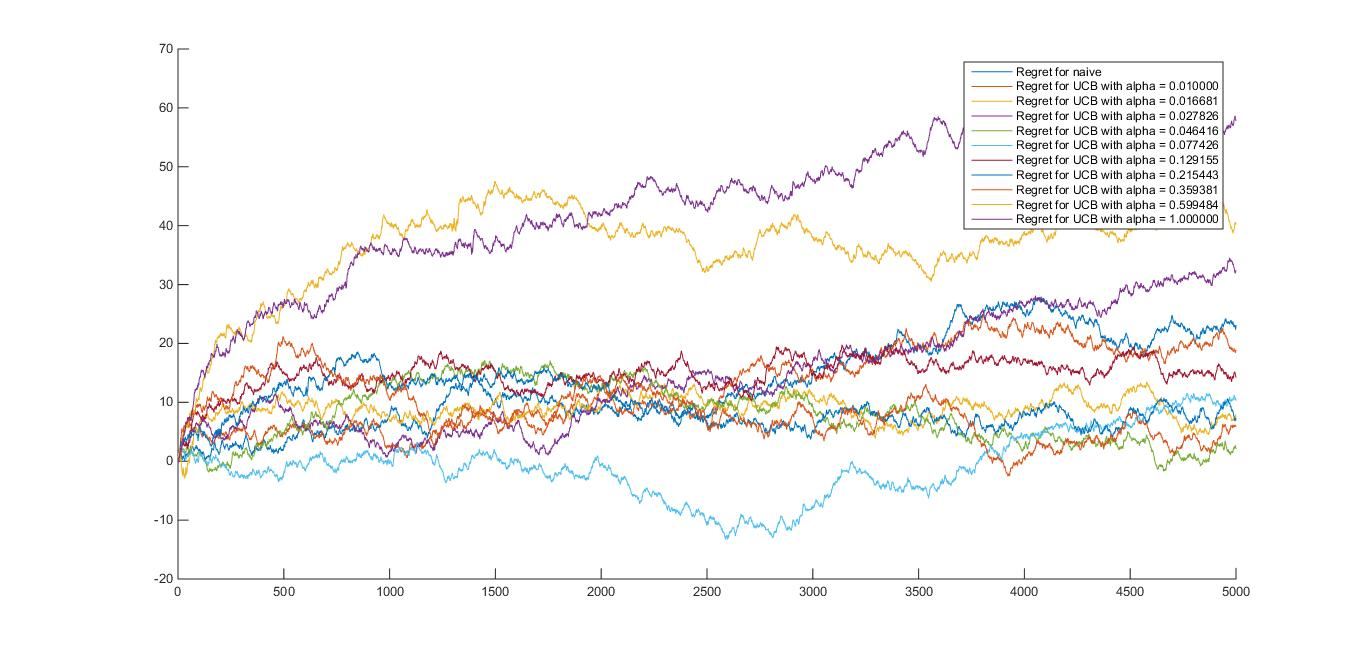
\includegraphics[scale=0.4]{regret_curves.jpg}
	\caption{Regret curves for the naive strategy and the UCB algorithm for several values of $\alpha$}
\end{figure}

\section{Complexity of a bandit problem}

We take a new MAB only composed of Bernoulli arms :
\begin{verbatim}
Arm5 = armBernoulli(0.2);
Arm6 = armBernoulli(0.24);
Arm7 = armBernoulli(0.55);
MAB_ber ={Arm1, Arm7, Arm5, Arm6};
\end{verbatim}

For this MAB, we find as value for the complexity $c = 6,23$.
We plot this lower bound and the regret curve :
\begin{figure}[H]
	\centering
	\noindent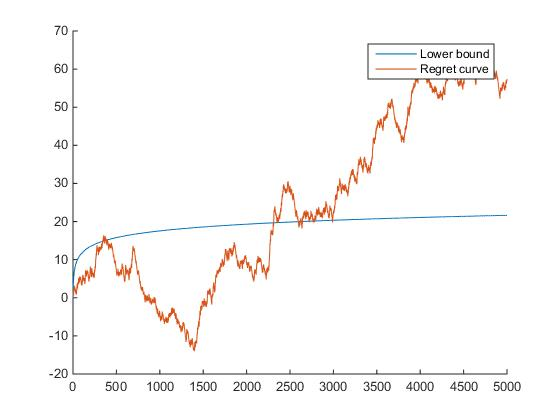
\includegraphics[scale=0.4]{complexity.jpg}
	\caption{Lower bound and regret curve}
\end{figure}

\section{A Bayesian idea for Bernoulli bandit problems}

\end{document}